\section*{Problem 1: Simple linear equation example}
\begin{enumerate}
\item Substituting (1a) into (1b), we get
        \begin{equation}\label{Q1_1}
        	a-b\cdot q=c+d\cdot q\implies
        	b\cdot q+d\cdot q-(a-c)=0.
        \end{equation}

\item Solving Eq.\eqref{Q1_1} for $q$,
        \begin{equation}
        	q=\frac{a-c}{b+d}.
        \end{equation}
      Substituting into (1a),
      	\begin{equation}
			p=a-b\cdot\frac{a-c}{b+d}.
		\end{equation}

\item Rearranging terms in the system,
		\begin{equation}
        	\begin{cases}
        		p+b\cdot q=a\\
        		p-d\cdot q=b
        	\end{cases}\implies
        	\underbrace{
            	\begin{pmatrix}
            		1	&	b\\
            		1	&	-d
            	\end{pmatrix}
        	}_{A}
        	\underbrace{
            	\begin{pmatrix}
            		p	\\	q
            	\end{pmatrix}
        	}_{x}=
        	\underbrace{
            	\begin{pmatrix}
            		a	\\	c
            	\end{pmatrix}
        	}_{y}.
        \end{equation}
      Applying the LU decomposition,
		\begin{enumerate}
        	\item Define $L\cdot U=A$, where
                      \begin{equation}
                      	L=
                		\begin{pmatrix}
                			1&0\\0&1
                		\end{pmatrix},\qquad
                		U=
                		\begin{pmatrix}
                			1&b\\1&-d
                		\end{pmatrix}.
                      \end{equation}
        		    Subtracting the first row from the second row,
            		  \begin{equation}
                      	L=
                		\begin{pmatrix}
                			1&0\\1&1
                		\end{pmatrix},\qquad
                		U=
                		\begin{pmatrix}
                			1&b\\0&-d-b
                		\end{pmatrix}.
                      \end{equation}
        	\item Solving $L\cdot b=y$,
        			\begin{equation}
        				\begin{pmatrix}
                			1&0\\1&1
                		\end{pmatrix}
        				\begin{pmatrix}
        					b_1\\b_2
        				\end{pmatrix}=
        				\begin{pmatrix}
        					a\\c
        				\end{pmatrix}\implies
        				\begin{cases}
        					b_1=a\\
        					b_1+b_2=c
        				\end{cases}\implies
        				\begin{cases}
        					b_1=a\\
        					b_2=c-a
        				\end{cases}
        			\end{equation}
        	\item Solving $U\cdot x=b$,
        			\begin{equation}
        				\begin{pmatrix}
                			1&b\\0&-d-b
                		\end{pmatrix}
        				\begin{pmatrix}
        					p\\q
        				\end{pmatrix}=
        				\begin{pmatrix}
        					a\\c-a
        				\end{pmatrix}\implies
        				\begin{cases}
        					p=a-b\cdot\dfrac{a-c}{b+d}\\
        					q=\dfrac{a-c}{b+d}
        				\end{cases}.
        			\end{equation}
		\end{enumerate}
    	\item Substituting $a=3,b=0.5,c=d=1$, we obtain
    		\begin{equation}
				\begin{cases}
					p^*=a-b\cdot\dfrac{a-c}{b+d}=\dfrac{4}{3}\\
					q^*=\dfrac{a-c}{b+d}=\dfrac{7}{3}
				\end{cases}.
			\end{equation}
\item The iteration method converges with order $(\mathbf D, \mathbf S)'$ but not the other way round. Convergence and non-convergence are illustrated graphically in Figure \ref{convergence} and \ref{nonconvergence} respectively.
        \begin{figure}[htbp]
        	\begin{center}
        		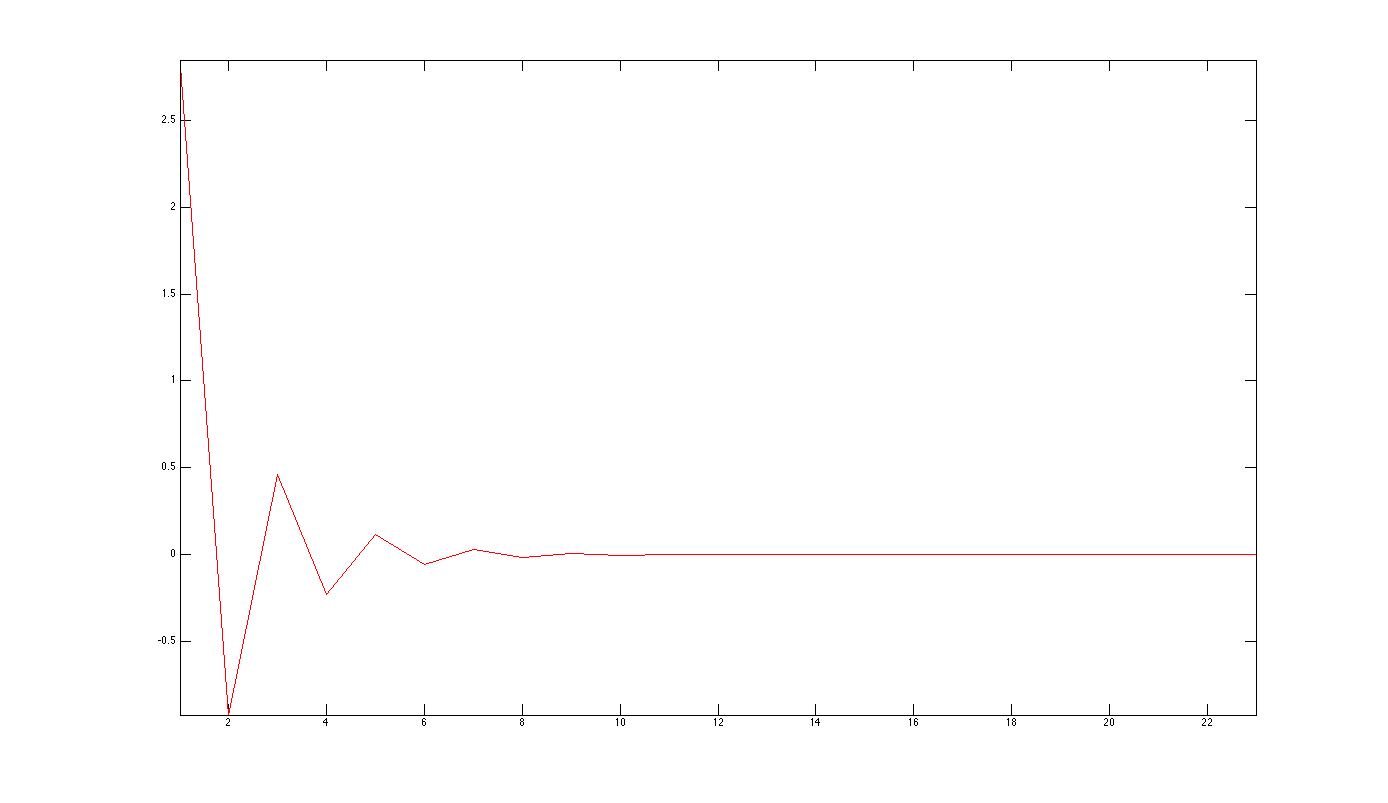
\includegraphics[width=12cm]{Plot/Q1/Convergence.png}
        		\caption{Convergence Case}
				\label{convergence}
			\end{center}
		\end{figure}
		\begin{figure}[htbp]
			\begin{center}
	        	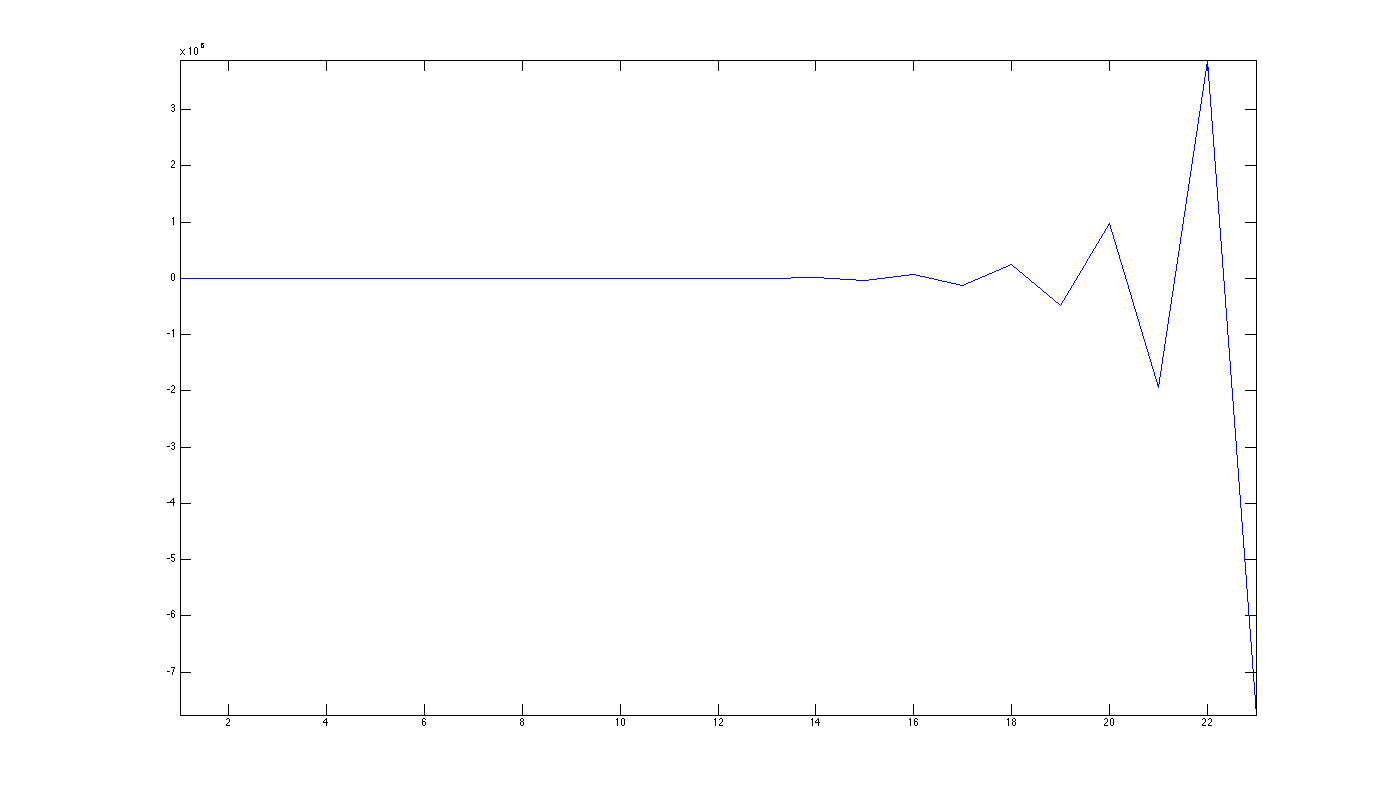
\includegraphics[width=12cm]{Plot/Q1/Nonconvergence.png}
        		\caption{Non-Convergence Case}
				\label{nonconvergence}
			\end{center}
        \end{figure}
\item The system does not converge for all of the $\lambda$ chosen.
\end{enumerate}
